\documentclass[fleqn, 10pt]{beamer}\usepackage[]{graphicx}\usepackage[]{color}
% maxwidth is the original width if it is less than linewidth
% otherwise use linewidth (to make sure the graphics do not exceed the margin)
\makeatletter
\def\maxwidth{ %
  \ifdim\Gin@nat@width>\linewidth
    \linewidth
  \else
    \Gin@nat@width
  \fi
}
\makeatother

\definecolor{fgcolor}{rgb}{0.345, 0.345, 0.345}
\newcommand{\hlnum}[1]{\textcolor[rgb]{0.686,0.059,0.569}{#1}}%
\newcommand{\hlstr}[1]{\textcolor[rgb]{0.192,0.494,0.8}{#1}}%
\newcommand{\hlcom}[1]{\textcolor[rgb]{0.678,0.584,0.686}{\textit{#1}}}%
\newcommand{\hlopt}[1]{\textcolor[rgb]{0,0,0}{#1}}%
\newcommand{\hlstd}[1]{\textcolor[rgb]{0.345,0.345,0.345}{#1}}%
\newcommand{\hlkwa}[1]{\textcolor[rgb]{0.161,0.373,0.58}{\textbf{#1}}}%
\newcommand{\hlkwb}[1]{\textcolor[rgb]{0.69,0.353,0.396}{#1}}%
\newcommand{\hlkwc}[1]{\textcolor[rgb]{0.333,0.667,0.333}{#1}}%
\newcommand{\hlkwd}[1]{\textcolor[rgb]{0.737,0.353,0.396}{\textbf{#1}}}%
\let\hlipl\hlkwb

\usepackage{framed}
\makeatletter
\newenvironment{kframe}{%
 \def\at@end@of@kframe{}%
 \ifinner\ifhmode%
  \def\at@end@of@kframe{\end{minipage}}%
  \begin{minipage}{\columnwidth}%
 \fi\fi%
 \def\FrameCommand##1{\hskip\@totalleftmargin \hskip-\fboxsep
 \colorbox{shadecolor}{##1}\hskip-\fboxsep
     % There is no \\@totalrightmargin, so:
     \hskip-\linewidth \hskip-\@totalleftmargin \hskip\columnwidth}%
 \MakeFramed {\advance\hsize-\width
   \@totalleftmargin\z@ \linewidth\hsize
   \@setminipage}}%
 {\par\unskip\endMakeFramed%
 \at@end@of@kframe}
\makeatother

\definecolor{shadecolor}{rgb}{.97, .97, .97}
\definecolor{messagecolor}{rgb}{0, 0, 0}
\definecolor{warningcolor}{rgb}{1, 0, 1}
\definecolor{errorcolor}{rgb}{1, 0, 0}
\newenvironment{knitrout}{}{} % an empty environment to be redefined in TeX

\usepackage{alltt}
\usepackage{amsmath}
\usepackage{amssymb}
\usepackage{geometry}
\usepackage{graphicx}
\usepackage{url}
\usepackage{xcolor}
\usepackage{enumerate}

% some latex magic for correcting apostrophe issue in verbatim mode
\makeatletter
\let \@sverbatim \@verbatim
\def \@verbatim {\@sverbatim \verbatimplus}
{\catcode`'=13 \gdef \verbatimplus{\catcode`'=13 \chardef '=13 }} 
\makeatother
\IfFileExists{upquote.sty}{\usepackage{upquote}}{}
\begin{document}

%---------------------------------------------
\begin{frame}
\large
Lecture 9:\\
Confidence Interval for One Mean\\
STAT 310, Spring 2021
\normalsize
\end{frame}

%---------------------------------------------
\begin{frame}{Introduction}
\begin{itemize}
\item Similar to how we can model the sample proportion $\hat{p}$ using a normal distribution, the sample mean $\bar{x}$ can also be modeled using a normal distribution when certain conditions are met.
\vspace{5pt}
\item However, we'll learn that a new distribution, called the $t$-distribution, tends to be more useful when working with the sample mean.
\vspace{5pt}
\item In this lecture we'll first learn about this new distribution, and then use it to construct confidence intervals for the mean.
\end{itemize}
\end{frame}

%---------------------------------------------
\begin{frame}{Central Limit Theorem (CLT) for the Mean}
\vspace{-2.5cm}
When the sample size $n$ is sufficiently large, the sampling distribution for $\bar{x}$ follows an approximate normal distribution centered around the population mean $\mu$, and with standard error $SE = \sigma / \sqrt{n}$
\end{frame}

%---------------------------------------------
\begin{frame}
% draw sampling distribution
\end{frame}

%---------------------------------------------
\begin{frame}
% draw sampling distribution
\end{frame}



% \begin{frame}
% \begin{itemize}
% \item One issue when applying the CLT is that the the standard error formula $SE = \sigma / \sqrt{n}$ is in terms of the population standard deviation $\sigma$, which is unknown.
% \item One solution is to plug in the sample standard deviation $s$ as the estimate of $\sigma$, so $SE \approx s  \sqrt{n}$ 
% \end{itemize}
% \end{frame}

%---------------------------------------------
\begin{frame}
%\small
\begin{itemize}
\item Based on the CLT, we can construct a 95\% confidence interval for the population mean $\mu$ as
$$\bar{x} \pm z^* SE \implies \bar{x} \pm 1.96 \frac{\sigma}{\sqrt{n}}$$
\item However, one issue with this confidence interval formula is that the standard error is in terms of the population standard deviation $\sigma$, which is unknown.
\item We can resolve this by plugging in the sample standard deviation $s$ as the estimate of $\sigma$.  That is, use $SE \approx s / \sqrt{n}$.  
\item This is a sensible approach when the sample size is large.  But when the sample size is small, the confidence interval needs to be adjusted to account for additional uncertainty in estimating $\sigma$ with $s$. 
\item It turns out that we can get a more accurate confidence interval, which accounts for this additional uncertainty, by using the $t$-distribution to calculate the critical value instead of the $z$-distrubiton.
\end{itemize}
\end{frame}

\begin{frame}{t-disribution}
\begin{itemize}
\item A $t$-distribution is bell-curve shaped distribution that is centered around zero.
\vspace{5pt}
\item It looks similar to a standard normal distribution, but it has wider tails.
\end{itemize}
\begin{figure}
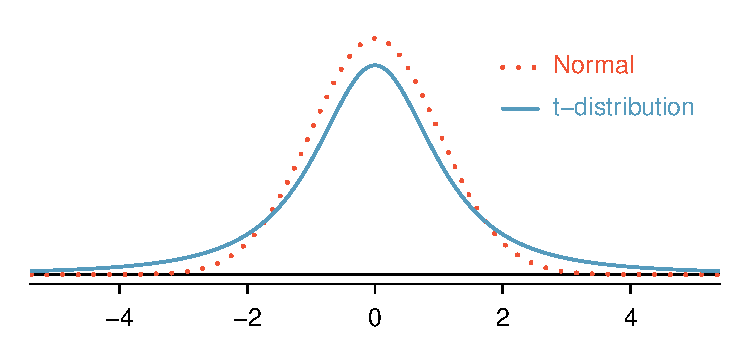
\includegraphics[scale = 0.6]{figure/tDistCompareToNormalDist.pdf}
\end{figure}
\end{frame}

\begin{frame}{t-disribution}
\begin{itemize}
\item The shape of the $t$-distribution depends on the degrees of freedom, which is defined as $df = n-1$
\item When the sample size is small the $t$-distrubiton has noticeably wider tails than a normal distribution.
\item When the sample size is large (about 30 or more), the $t$-distribution is nearly identical to a normal distribution.
\end{itemize}
\begin{figure}
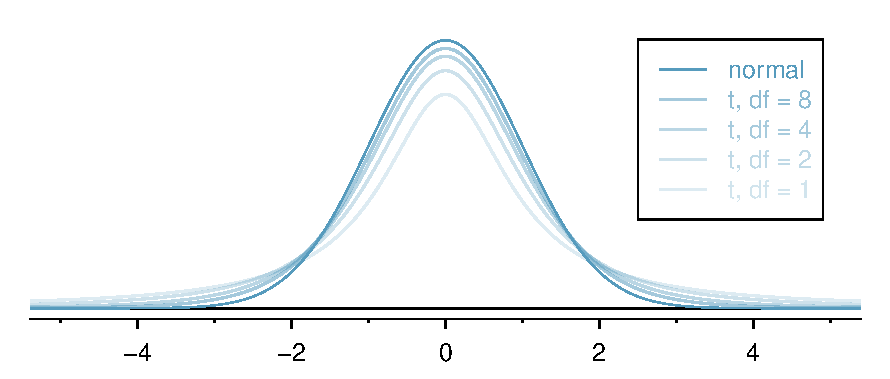
\includegraphics[scale = 0.5]{figure/tDistConvergeToNormalDist.pdf}
\end{figure}
\end{frame}

\begin{frame}{Confidence Interval for $\mu$}
A confidence interval for the the population mean $\mu$ is given by 
$$\bar{x} \pm t^* \frac{s}{\sqrt{n}}$$\\
\vspace{1cm}

The critical value $t^*$ is found using $t$-distribution.  It depends on the confidence level and degrees of freedom, and can be computed using the R function \texttt{qt()}.\\
\bigskip

\emph{Example}: Calculate the critical value $t^*$ when the confidence level is $95\%$ and $n=15$.
\vspace{2cm}

\end{frame}

\begin{frame}{Confidence Interval for $\mu$}
The confidence interval formula is valid if the following conditions are satisfied:
\vspace{5pt}
\begin{itemize}
\item The data come from a random sample.  (This is called the \textbf{independence condition} in the textbook.)
\vspace{5pt}
\item The sample size $n$ is large ($n \geq 30$).  Otherwise, if the sample size is small ($n < 30$), the data should have an approximate normal distribution. (This is called the \textbf{normality condition} in the textbook.)
\vspace{5pt}
\item Additionally, the data should not contain any extreme outliers.
\end{itemize}
\vspace{5pt}
Graphical methods (box plots, histograms) can be used to check if the data have an approximate normal distribution when the sample size $n$ is small.
\end{frame}

\begin{frame}{Example}
\vspace{-1cm}
\small
Below are some summary statistics and a box plot for the ages of a random sample of $n=26$ female athletes who participated in the 2012 Olympic Games in London.  Calculate and interpret a 95\% confidence interval for the population mean age.  Also comment on whether the conditions for the confidence interval appear satisfied.
\begin{table}[ht]
\begin{tabular}{lllll}
\hline
n & $\bar{x}$ & s & min & max\\
\hline
26 & 26.9 & 4.5 & 19 & 36
\end{tabular}
\end{table}
\vspace{-0.5cm}
\begin{figure}
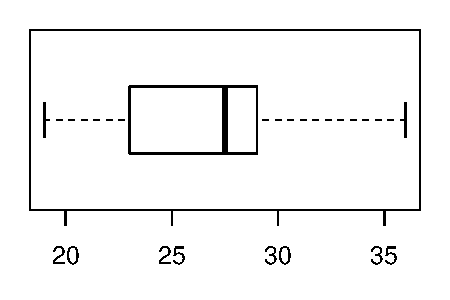
\includegraphics[scale=0.5]{figure/age_boxplot.pdf}
\end{figure}
\end{frame}

\begin{frame}
\end{frame}

\begin{frame}{Example}
\vspace{-4cm}
Calculate and interpret a 99\% confidence interval for the population mean age of female athletes who participated in the 2012 Olympic Games.
\end{frame}



\end{document}
